% \section{Software Requirements Specification}

\section{Einführung}

\subsection{\textbf{Zweck}}
Dieses Dokument dient als Grundlage zur Beauftragung des berufsbegleitenden Studienganges, Kommunikations- und Medieninformatik des Matrikel 13, mit der Programmierung einer \acs{HfTL}-\acs{APP}. Es setzt dabei die Rahmenbedingungen fest.

\subsection{\textbf{Hintergründe und Ziele des Projekts}}
Die \acf{HfTL} ist eine private, staatlich anerkannte Fachhochschule. Träger der \ac{HfTL} ist die \ac{HfTL}-Trägergesellschaft \acs{mbH}, eine Beteiligungsgesellschaft der Deutschen Telekom AG. Die Schule befindet sich im Leipziger Stadtteil Connewitz. Es werden sowohl Direkt- als auch duale Studiengänge und berufsbegleitende Studiengänge angeboten.
Aufgrund des umständlichen Beschaffens der Noten und Stundenpläne sowie der Termine für Teletutorings, wird eine Smartphone-Applikation benötigt. Diese stellt ein Benutzerinterface für Studenten der \acs{HfTL} dar, mit dem der Zugriff auf die im \acs{QIS} hinterlegten Daten vereinfacht.

\subsection{\textbf{Produktumfang}}

Der Betrieb der \acs{HfTL}-APP muss auf allen gängigen Android-Smartphones ab Version 4.0 möglich sein.

Durch die APP wird den Studenten der HFTL ermöglicht: 

\begin{itemize}
      \item die aktuellsten Nachrichten der \acs{HfTL}-Webseite lesen
      \item auf \acs{QIS} zugreifen
      \item Studenten sollen ihre(-n) Noten(-spiegel) aufrufen können
      \item Vorlesungspläne zu lesen
      \item Raumbelegungspläne abzurufen
\end{itemize}
   
Zusätzlich werden folgende Anforderungen gestellt:

\begin{itemize}
	\item Erweiterbarkeit für weitere Funktionen und Anwender
	\item spätere IOS-Version
\end{itemize}


\subsection{\textbf{Musskriterien}}

Zunächst müssen zwingend folgende Punkte des Umfangs erfüllt werden:

\begin{itemize}
   	\item NEWS
   	\item NOTEN
   	\item STUNDENPLAN   
\end{itemize}

\subsection{\textbf{Abgrenzungskriterien}}

Die \acs{APP} soll später auch für zusätzliche Informationen, wie ein Raumplanung erweiterbar sein. Eine spätere Version für IOS-Geräte ist ebenfalls geplant, ist hier aber nicht Bestandteil.				

\subsubsection{Kostenrahmen}

Für die Entwicklung der \acs{APP} soll auf kostenfreie Opensource-Programme oder auf vordefinierte Klassen der Programmierung zurückgegriffen werden.
Außer den personellen Aufwand dürfen keine Zusätzlichen Kosten entstehen.


\subsection{\textbf{Definitionen, Akronyme, Abkürzungen}}
\begin{acronym}[UV-Licht]
\acro{HfTL}{Hochschule für Kommunikation Leipzig}
\acro{APP}{Kurzform für Applikation}
\acro{mbH}{mit beschränkter Haftung}
\acro{QIS}{Qualitätssteigerung der Hochschulverwaltung im Internet durch Selbstbedienung}
\acro{iCal}{Datenformat zum Austausch von Kalenderinhalten}
\acro{SoSe15}{Sommersemester 2015}
\acro{XML}{ Extensible Markup Language}
\acro{HTTPS}{HyperText Transfer Protocol Secure}
\acro{AES}{Advanced Encryption Standard}
\acro{SQL}{Structured Query Language}
\acro{.apk}{Android application package}
\acro{MTBF}{mean time between failure}
\acro{CI/CD}{Corperate Identity/Corperate Design}

\end{acronym}

\subsection{\textbf{Referenzen}}

\begin{itemize}		
	\item QIS-System:  \url{https://qisweb.hispro.de/tel/rds?state=user&type=0} 
	
	\item News der HfTL  \url{https://www.hft-leipzig.de/de/studierende/service/news.html}	
\end{itemize}


\section{Allgemeine Übersicht}

\subsection{\textbf{Beschreibung der Ausgangssituation (Ist-Zustand) }}

Damit Studenten auf \acs{QIS} zugreifen kann, müssen diese sich über einen Browser auf der \acs{QIS}-Seite einloggen und über das unübersichtliche Menü ihre Daten suchen.
Studenten haben die Möglichkeit ihre Noten oder einen Notenspiegel einzusehen.
Für IPhone-Nutzer gibt es bereits eine kostenpflichtige \acs{APP} , namens Grades, die Noten und Informationen über die angemeldete Prüfungen auslesen kann.
Um die auf \acs{QIS} hinterlegten Vorlesungspläne abzurufen ist kein Login erforderlich, jedoch ist es notwendig sich umständlich zu dem entsprechenden Studiengang zu navigieren. Einzelne Vorlesungen oder Stundenpläne können als \acs{iCal} heruntergeladen werden.
Ebenso sind die Teletutorien hier zu finden.
Die aktuellen Nachrichten der Hochschul-Homepage sind auf einer anderen Seite zu finden, welche öffentlich zugänglich ist.


\subsection{\textbf{Produkteinsatz}}

\subsubsection{Anwendungsbereiche}
Aktuell soll die APP nur für die Studenten der \acs{HfTL} zugänglich sein, welche ein Android-Smartphone besitzen. 

\subsubsection{Zielgruppen, Qualifikationsniveau}

Da bei der Nutzergruppe von Studenten mit Erfahrung im Umgang mit solchen APP's ausgegangen werden kann, wird auch die Oberfläche dementsprechend gestaltet.

\subsection{\textbf{Produktfunktionalität}}

Die APP soll sich mittels regelmäßiger Abfragen der \acs{HfTL}-Homepage, sowie von \acs{QIS}, die News, Noten und Stunden- und ggf. Raumbelegungspläne ziehen und die Noten für den Nutzer lokal auf dem Smartphone speichern und entsprechend darstellen. 
Es soll sichergestellt werden das auf sensible Daten wie z.B. Noten auch nur autorisierte Nutzer Zugang bekommen. Die APP soll in deutscher Sprache dargestellt werden. Evtl. wird sie im Nachgang in andere Sprachen übersetzt. 

\subsection{\textbf{Randbedingungen}}

Der zeitliche Rahmen für die Entwicklung und Programmierung dieser APP begrenzt sich auf das \ac{SoSe15} und dem Studienmodul Software-Engineering.
Für die Entwicklung dieser APP, sowie Vertrieb, Programmierung usw. dürfen keine Kosten entstehen.
Supportleistungen werden in der Projektphase über das Projektteam geleistet. Die Wartung wird, bis mit der Veröffentlichung die APP der Hochschule kostenfrei zur Verfügung gestellt wird, ebenfalls vom Projektteam übernommen. Die Dokumentation wird ebenfalls vollständig an die Hochschule übergeben.
Durch das Projektteam wird es keine weitere Softwarebetreuung, Wartung oder der gleichen geben. Es finden ebenfalls keine Schulungen oder Einweisungen statt.

\subsection{\textbf{Annahmen und Abhängigkeiten}}

Die APP wird für Android-Geräte ab Version 4.0.3 zur Verfügung stehen.
Entsprechend der Vorgaben der Deutschen Telekom AG muss bei der Programmierung der APP, explizit beim Design, auf die Konzernrichtlinien geachtet werden. Es soll zusätzlich auf die Designempfehlungen für Androidgeräte geachtet werden.

\subsection{\textbf{Verzögerungen}}

Durch die strikte Abtrennung des zeitlichen Rahmens auf das \acs{SoSe15} darf es über diesen Zeitraum hinaus nicht zu Verzögerungen kommen

\section{Anwendungsszenarien}

\subsection{\textbf{Beschreibung aus der Nutzersicht}}

Die Benutzeroberfläche muss intuitiv bedienbar sein. Der strukturierte Aufbau durch Kategorien (News, Noten, Stundenplan) soll die Übersichtlichkeit erhöhen.
Die Logindaten werden verschlüsselt auf dem Smartphone gespeichert und auch verschlüsselt übertragen.
Durch eine durchgehende und vollständige Dokumentation soll eine Wartung auch durch spätere Matrikel oder Administratoren der Hochschule möglich sein.
Eine Implementierung weiterer Funktionen soll auch im Nachhinein möglich sein.

\section{Anforderungen}

\subsection{\textbf{Fachkonzept}}
Die \acs{HfTL}-APP  wird in Java programmiert um durch Verwendung bestehender Klassen die Erweiterbarkeit und Realisierbarkeit zu vereinfachen. Für das Design werden \acs{XML}-Stylesheets verwendet.
Pull-und Push-Service werden zur Benachrichtigung und Abfrage verwendet.




\subsubsection{Überblick über das Gesamtsystem}
$\;$ \\ %Zeilenumbruch bei Nutzung von paragraph

\textbf{Noten}
\begin{itemize}
	\item die APP soll die Noten lokal auf dem Smartphone nach Semester aufgeschlüsselt anzeigen
	\item Login über die APP
	\item Anmeldung über gesicherte, verschlüsselte Übertragung (\acs{HTTPS})
	\item verschlüsselte Speicherung der Daten auf dem Smartphone (\acs{AES})
	\item verschlüsselte Speicherung der Daten auf dem Smartphone (\acs{AES})
	\item Pull-Nachrichten (Einstellbares Intervall und/oder manuell)
	\item Push-Benachrichtigung
	\item Nutzer wird mit Hinweismeldung informiert, wenn Noten aktualisiert wurden
\end{itemize}
Optionale Angaben im Menüpunkt Noten:
\begin{itemize}
	\item Klassenspiegel
	\item Notenverteilung
	\item Anzahl der Teilnehmer
	\item Notenschnitt
	\item Anzeige der Creditpoints
	\item zu erreichende Creditpoints
	\item erreichte Creditpoints
\end{itemize}
\textbf{Stundenpläne}
\begin{itemize}
	\item Stundenplan nur für zum Nutzer passenden Studiengang
	\item Pull-Nachrichten (Einstellbares Intervall und/oder manuelle Abfrage)
	\item Synchronisierung mit dem Kalender auf dem Smartphone	
\end{itemize}
\textbf{News}
\begin{itemize}
	\item Pull-Nachrichten (manuelle Aktualisierung)
	\item News von: \url{https://www.hft-leipzig.de/de/studierende/service/news.html}
\end{itemize}



\subsubsection{Verwendete Bibliotheken von Drittanbieteren}
\begin{itemize}
	\item jsoup 1.8.1 – MIT-Lizenz
	\item iCal4j 1.0.6 – BSD-Lizenz 
\end{itemize}


\subsection{\textbf{Anforderungen an die Datenhaltung}}

Alle gespeicherten Daten müssen vor unbefugtem Zugriff geschützt werden, dafür werden Benutzerdaten in einer \acs{SQL}-Datenbank gespeichert und durch das Passwort und den Benutzernamen freigegeben. Passwort und Benutzername wurden mit \acs{AES} verschlüsselt.

\subsubsection{allgemeine Beschreibung der Daten}
Sicherheitsrelevante Daten sind in dem Notenteil der App zu finden. Diese sind der Benutzername, das Passwort, die Prüfungs- und Prüfungsvorleistungsergebnisse, der Klassenspiegel und die Creditpoints.
Die öffentlichen Daten sind in den anderen beiden Teilen der App enthalten.
Dazu gehören die News mit ihren Terminen und Inhalt und der Stundenplan mit den Veranstaltungen und den dazugehörenden Informationen wie Dozent und Veranstaltungsort.


\subsection{\textbf{Anforderungen an die Benutzeroberfläche}}

\subsubsection{allgemeine Anforderungen an die Oberfläche}

Das Layout richtet sich nach dem  \ac{CI/CD} der Deutschen Telekom AG, speziell dem der \acs{HfTL} Trägergesellschaft, stand 14.12.12. Entsprechend sind primär die Farben, sowie Schriftarten vorgegeben. Das Layout zieht sich einheitlich (mit funktionsbedingten Abweichungen) durch alle APP-Teile und soll eine leichte Bedienung begünstigen.
Die Größe der einzelnen Elemente (Buttons, Zeilen, Überschriften etc.) ist an den Designempfehlungen seitens Android angelehnt. 
Auch die Abstände zwischen den einzelnen Elementen wurden – sofern sie mit dem \ac{CI/CD} in Einklang stehen – entsprechend der Designempfehlung festgelegt.
Die Reaktionszeit der Benutzereingaben soll mit möglich wenig Verzögerung verarbeitet und dargestellt werden.






\subsubsection{Berechtigungen}

Die APP wird als Open Source bereitgestellt.

Nicht angemeldete Benutzer können sich die News und den Stundenplan anzeigen lassen. Angemeldete Benutzer können zusätzlich ihre Noten abrufen.

Die App braucht folgende Berechtigung auf dem Smartphone:
\begin{itemize}
	\item Netzwerkstatus abrufen: zur Kontrolle ob das Handy online ist
	\item Internet: APP greift auf das Internet zu
	\item Telefonstatus: wird zur Verschlüsselung benötigt
\end{itemize}




\subsubsection{Bildschirmlayout}
siehe Anhang \ref{subsec:App-Layout}





\subsubsection{Dialogstruktur, Dialogabläufe}
\textcolor{magenta}{Maik/Stefan bitte hier Screenshots der jeweiligen Dialoge einfügen oder in Anhang unter Dialogmasken}





\subsection{\textbf{Leistungsanforderungen}}
Es wird von einer maximalen Nutzerzahl von 1000 Studenten ausgegangen.
Die Reaktionszeit/Programmstart der APP soll möglichst gering gehalten werden.
Das Datenaufkommen soll möglichst gering ausfallen.


\subsection{\textbf{Anfordeungen für Inbetriebnahme und Einsatz}}

\subsubsection{Sicherheitsziele}
Der Benutzername und das Passwort werden in einen gesicherten Speicherbereich (nur root), mit \acs{AES} verschlüsselt, gespeichert.
Die Datenbank in der die Noten gespeichert werden, liegt ebenfalls in diesem Bereich und darf nur von der \acs{HfTL}-App geöffnet werden.
Die Kommunikation mit der \acs{HfTL}-Website und \acs{QIS} erfolgt gesichert per \acs{HTTPS}.



\subsubsection{Installationsprozedur}

Der Wirkbetrieb soll nach Möglichkeit über den Android-Playstore realisiert werden. Falls es dabei zu Lizenz- und Kostenproblemen kommt, wird die APP als \ac{.apk} über die HfTL-Homepage verteilt.



\subsubsection{Pilot- bzw. Probebetrieb}
\textcolor{magenta}{Hier müssen die Versionsmanagementprotokolle rein!}




\subsubsection{Fehlerreaktion, Garantie, Service, »Wiederanlauf«}
Die Zuverlässigkeit sollte sich durch eine große \ac{MTBF} darstellen.



\subsubsection{Schulungen}
Nach Beendigung des Projektes werden keine Schulungen usw. durchgeführt.


\subsection{\textbf{Qualitätsanforderungen}}

\subsubsection{Qualitätsmerkmale}
Folgende Qualitätsansprüche werden gestellt:
\begin{itemize}
	\item Hohe Zuverlässigkeit der Software
	\item schnelle und zuverlässige Verarbeitung der gewünschten Daten
	\item sichere Datenspeicherung u. -übertragung mittels entsprechender Verschlüsselung
	\item Fehler werden mit einer entsprechenden Fehlermeldung beantwortet
	\item Intuitiv benutzbar
	\item Leicht zu warten und zu erweitern
	\item Vollständige Dokumentation des Projektes
\end{itemize}




\subsubsection{Qualitätssicherung}
Zur Qualitätssicherung werden einheitliche Testprotokolle und die entsprechenden Testkriterien erstellt. Es finden regelmäßige Kontrollen durch die Qualitätssicherung statt, um die Einhaltung der gegebenen Standards zu überprüfen. Es findet ebenfalls eine regelmäßige Kontrolle der Dokumentation statt. Die jeweiligen Software-Prototypen werden nach der Prototypisierung zur Fehlererkennung und zum Funktionstest an das Projektteam geschickt. Zur Verbesserung der Software werden die Tests anhand vorgegebener Testkriterien durchgeführt, um standardisierte Testergebnisse zu erhalten. Die Testergebnisse werden zur Auswertung an die entsprechende Projektgruppen zurück gespiegelt.


\subsubsection{Qualitätsnachweise}
Während des Projektzeitraumes werden sämtliche Meeting, Tests und Kontrollen protokolliert und zur Dokumentation in einem dafür vorgesehen Bereich abgelegt. Die gesetzten Standards und Vorgaben werden eingehalten. Zum Projektabschluss ist der geplante Umfang erreicht und alle Muss-Kriterien sind enthalten. Die APP ist funktionstüchtig.



\subsubsection{Offenlegung der Qualitätskontrollpläne}

\begin{tabular}{lll}
	\textbf{Nr.} & \textbf{Anforderung} & \textbf{Verantwortliche} \\
	1 & Projektrahmen festlegen & gesamtes Team \\
	1.1 & Projektrahmen festlegen & gesamtes Team \\
	1.2 & Architektur & gesamtes Team \\
	1.3 & Vorgehensmodell & gesamtes Team \\
	\\
	1 & Vollständige Dokumentation & gesamtes Team \\
	1.1 & UML Diagramme erstellen & AD, CM \\
	1.2 & Installationsanleitung und Benutzerhandbuch erstellen & GE, JS \\
	1.3 & Lasten- Pflichtenheft erstellen & SK, SC \\
	1.4 & Protokolle & ML, PK \\
	1.5 & Dokumentation zusammenstellen und gestalten & JS, SC \\
	\\
	2 & App erstellen & gesamtes Team \\
	2.1 & Design nach HfTL-Vorgaben erstellen & ML, SC \\
	2.2 & Programmierung der APP & GE \\	
	\\
	3 & Qualitätskontrolle & gesamtes Team \\
	3.1 & Testkriterien festlegen & PK \\
	3.2 & Testprotokollelayout erstellen & ML \\
	3.3 & Softwaretests & ML, PK \\
	3.4 & Kontrolle der Dokumentation & PK \\
	\\
	4 & Anfertigen der Präsentation & gesamte Team \\
	4.1 & Präsentation halten & SC, ML, SK, JS \\
\end{tabular}



\subsubsection{Berichte, Protokolle zum Nachweis des Vorgehens gemäß der Qualitätskontrollpläne}
Es liegen bei:
\begin{itemize}
	\item Sitzungsprotokolle etc. (siehe Anlagen)
\end{itemize}



\subsection{\textbf{Anforderung an die Entwicklung}}

\subsubsection{Entwicklungs-Umgebung}
Für die Entwicklung wird Android Studio inkl. Gradle in der Version 1.x genutzt. Für die Dokumentation und Projektkoordination wird GitHub verwendet.
Die Dokumentation wird mittels \LaTeX{} erstellt.



\subsubsection{Projekt-Organisation}
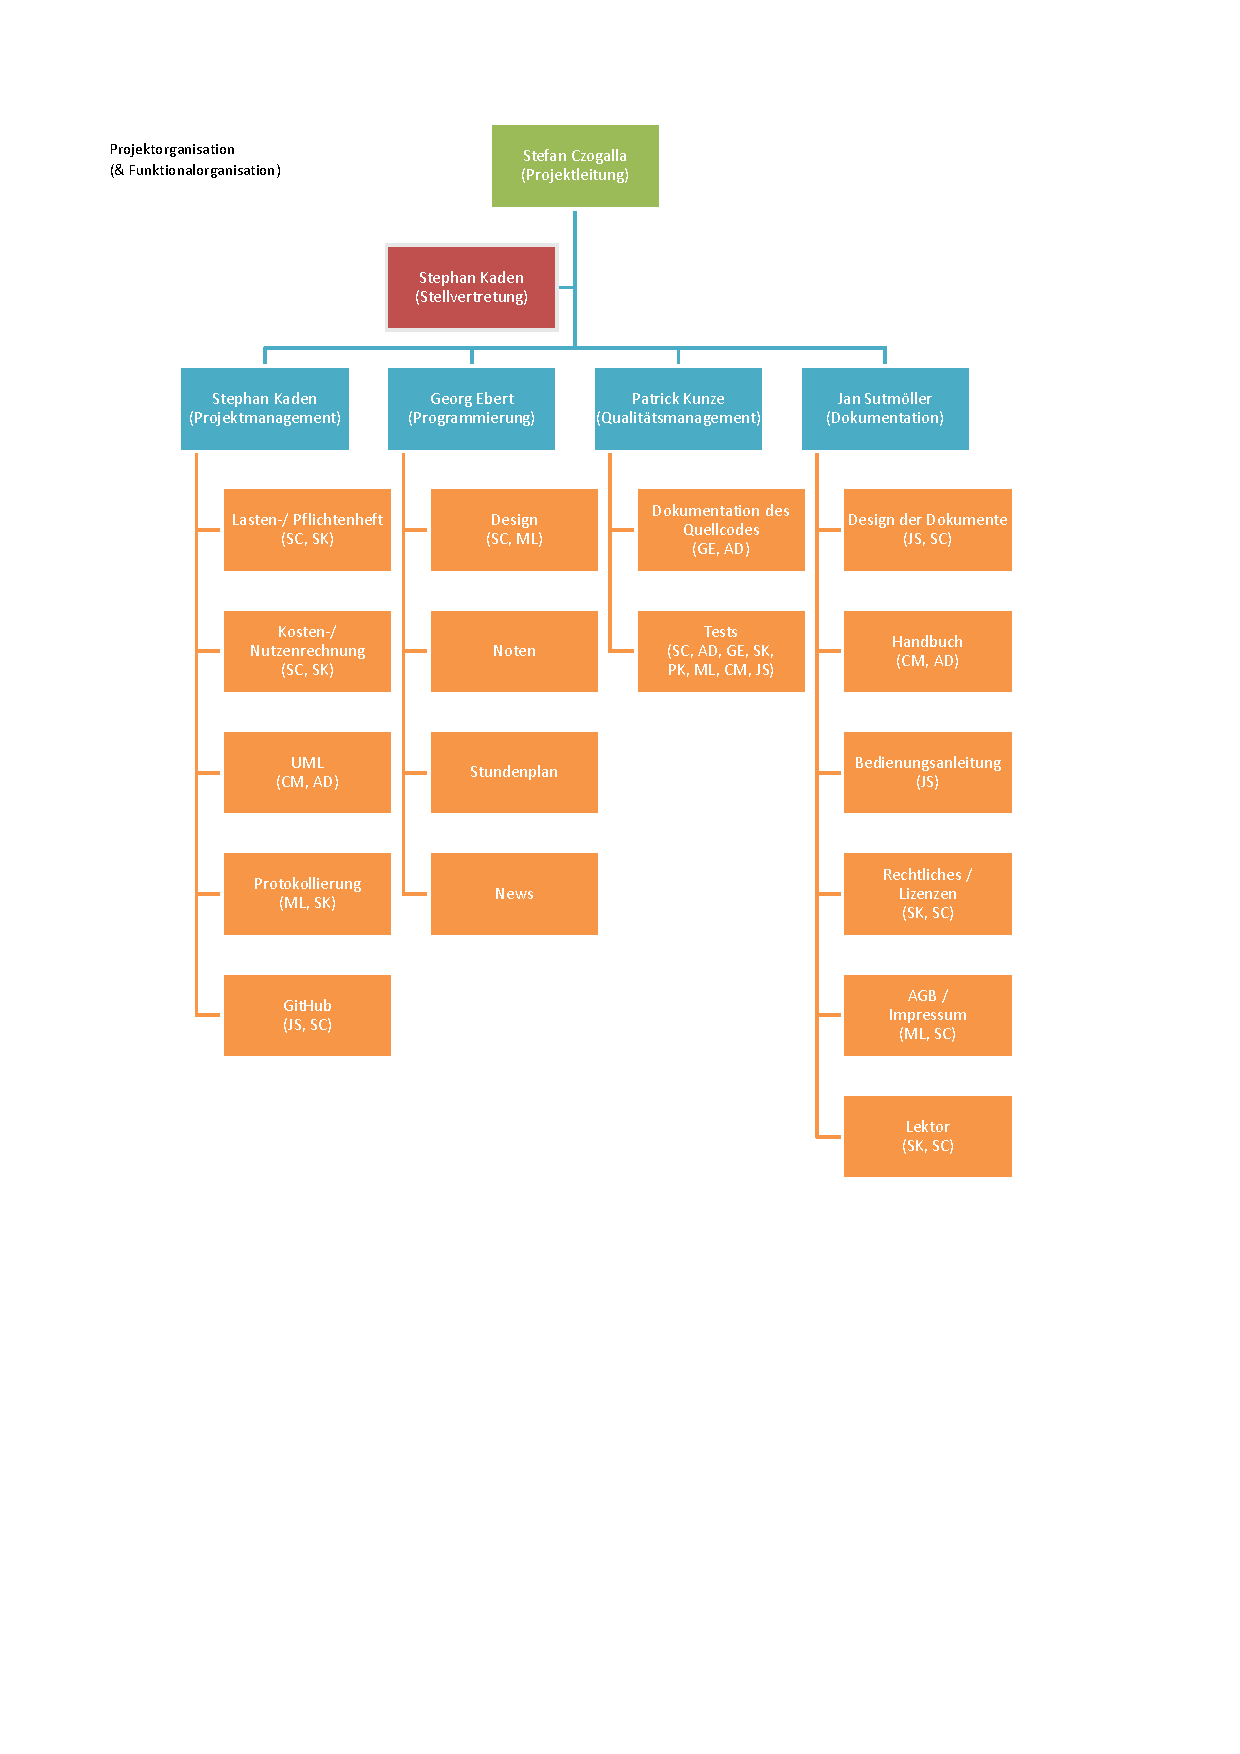
\includepdf[pages=-,noautoscale]{04_Anhang/files/swe_organigramm.pdf}


\subsubsection{Projekt-Planung}
\textcolor{magenta}{Verweis auf Projektstrukturplan im Anhang}

\subsubsection{Änderungsmanagement}
\textcolor{magenta}{GitHub Plan????}

\subsubsection{Testanforderungen}
siehe Anhang \ref{subsec:Testprotokollentwurf}



\section{Anhang}

\textcolor{magenta}{
\begin{itemize}
	\item Dialogmasken
	\item Dokumente
	\item Liste der Softwarelieferungen
	\item Projektorganigramm
	\item Projektstrukturplan
	\item Haupt-Termindaten
\end{itemize}
}